\documentclass{scrartcl}

\usepackage{vhistory}  % version history at end of document
\usepackage{hyperref}  % hyper references

\usepackage{graphicx}
\graphicspath{ {./Images/} }

\newcommand{\docTitle}{Setup Ubuntu Virtual Machine}
\newcommand{\MEK}{Matt Kontz}

\hypersetup{%
 	pdftitle = {\docTitle},
	pdfkeywords = {\docTitle, Version \vhCurrentVersion
	from \vhCurrentDate},
	pdfauthor = {\vhListAllAuthorsLong}
}

\usepackage{scrpage2}
\pagestyle{scrheadings}
\ihead{\docTitle\ -- Version \vhCurrentVersion}
\chead[]{}
%\ohead[\thepage]{\thepage}
%\ifoot{\docTitle\ -- Version \vhCurrentVersion}
\cfoot[\thepage]{\thepage}
%\ofoot[\thepage]{\thepage}

\begin{document}

\title{\docTitle}
\author{\vhListAllAuthors}
\date{Version \vhCurrentVersion\ from \vhCurrentDate}
\maketitle

\section{Summary}
This document was created to briefly described the steps required to setup a Ubuntu VirtualBox virtual machine in a windows host.




\section{Create Ubuntu Virtual Machine}
\label{sec:create_vm}

Create a VM with desire version of Linux 

\begin{enumerate}
	\item If required update or install VirtualBox in host  (e.g. Windows)
	\item On host (e.g. windows) download .iso image of desired version of Ubuntu (e.g. 16.04 or 18.04) \href{http://releases.ubuntu.com/16.04/}{releases.ubuntu.com/16.04/}
	\item From VirtualBox start a new virtual machine (VM) selecting desired memory, size, etc. once it starts select the .iso image with the desired version of Ubuntu. (Figures \ref{fig:Processor} - \ref{fig:Display})
	
	\begin{figure}[p]
		\centering
		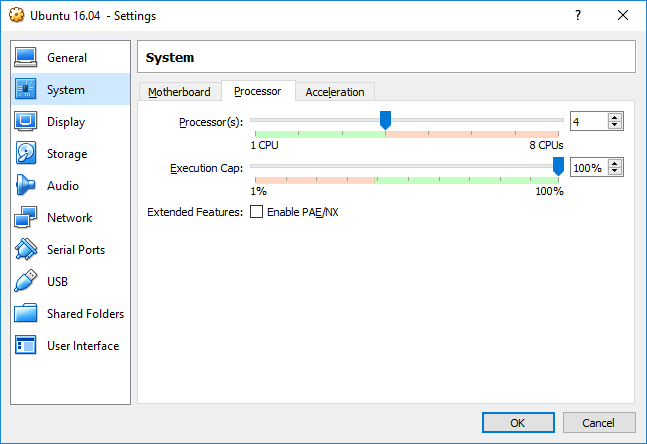
\includegraphics[width=3.0in]{Processor.png}
		\caption{Set number of processors for VM.}
		\label{fig:Processor}
	\end{figure}
	
	\begin{figure}[p]
		\centering
		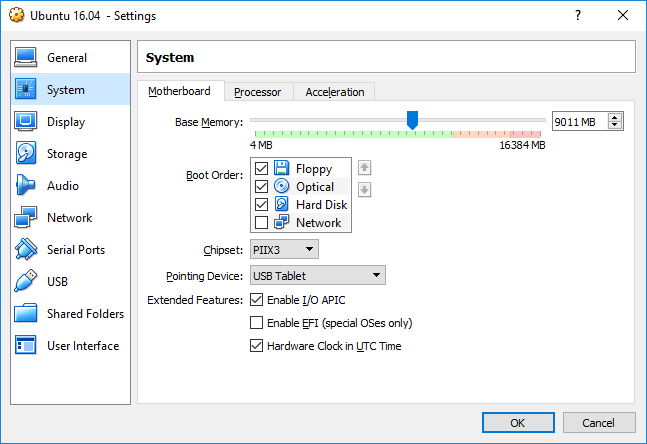
\includegraphics[width=3.0in]{Memory.png}
		\caption{Set amount of memory for VM.}
		\label{fig:Memory}
	\end{figure}

	\begin{figure}[p]
		\centering
		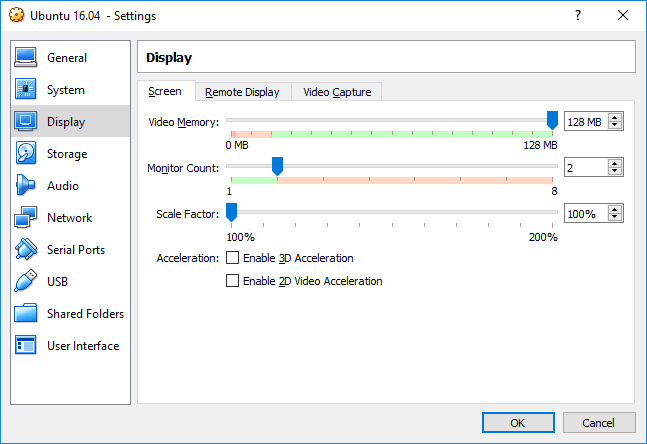
\includegraphics[width=3.0in]{Display.png}
		\caption{Set number of displays for VM.}
		\label{fig:Display}
	\end{figure}
	
	\item Follow directions to install Ubuntu on VM
	\item $[optional]$ Add terminal to launcher and customize launcher shortcuts
	\item Update Ubuntu $>>$ sudo apt-get update
	
\end{enumerate}

\section{Install Guest Addition on VM}
\label{sec:guest_additions}

Installing guest addition will help the Ubuntu VM integrate properly with Windows so that things like swap folders and copy/paste (text and images) work seamlessly between the Windows and the VM.

\begin{enumerate}
	\item Update Ubuntu: \\ $\qquad >>$ sudo apt-get update
	\item Download version of guest extension corresponding to version of  VirtualBox on the VM.
	\begin{itemize}
		\item \href{http://download.virtualbox.org/virtualbox/}{download.virtualbox.org/virtualbox/}
		\item \href{http://download.virtualbox.org/virtualbox/5.2.22/}{download.virtualbox.org/virtualbox/5.2.22/}
	\end{itemize}
	\item Mount disk image.  Run it and follow directions
	\begin{itemize}
		\item Right-click on .iso 
		\item select: ``Open With" $\rightarrow$ ``Disk Image Mounter"
		\item click run on pop-up
	\end{itemize}
	\item Update software: \\ $\qquad >>$ sudo apt-get update
	\item Setup swap directory: (Figure \ref{fig:swap}) \\ $\qquad >>$	sudo adduser $<$yourUsername$>$ vboxsf
	
	\begin{figure}[p]
		\centering
		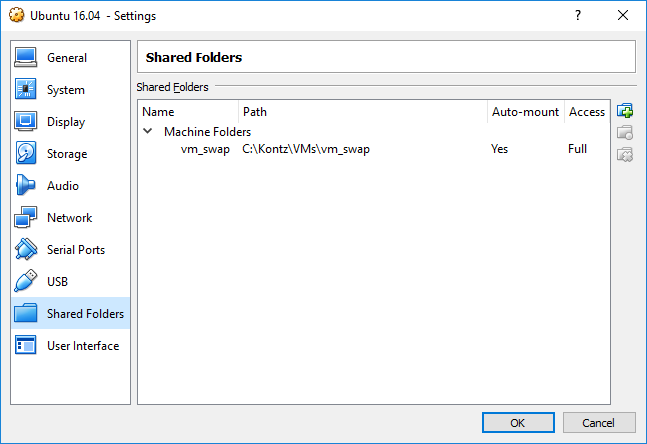
\includegraphics[width=3.0in]{swap.png}
		\caption{Set swap direction to pass files between host and VM.}
		\label{fig:swap}
	\end{figure}

	\item Close VM after installing guest additions.
	\item If it does exist add the desire swap folder on the host (e.g. Windows)
	\item Add desired swap folder in VM settings
	\item Enable directional clipboard in VirtualBox setting for VM on host. (Figure \ref{fig:Bidirectional})
	
	\begin{figure}[p]
		\centering
		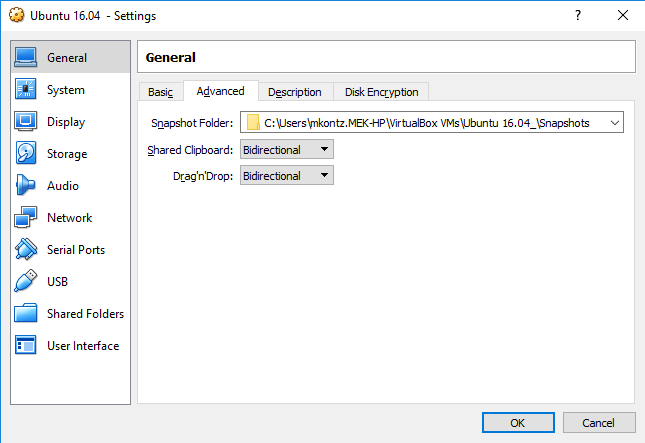
\includegraphics[width=3.0in]{Bidirectional.png}
		\caption{Set up directional host/VM clip-board.}
		\label{fig:Bidirectional}
	\end{figure}	

	\item Start VM
	\item Verify that swap directory is visible in Ubuntu VM and copy paste (images and text) should work in both directions. (Figure \ref{fig:sf_vm_swap})
	
	\begin{figure}[p]
		\centering
		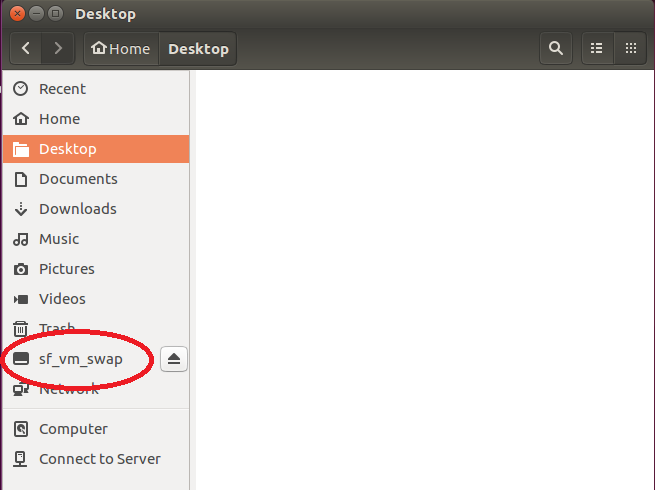
\includegraphics[width=3.0in]{sf_vm_swap.png}
		\caption{The swap folder in the VM will have the same name as the host folder with an ``sf\_" prefix.}
		\label{fig:sf_vm_swap}
	\end{figure}
	
\end{enumerate}

\section{Install Other Software}
\label{sec:guest_additions}

\begin{itemize}
	\item Update software: \\ $\qquad >>$ sudo apt-get update
	\item Install chrome
	\begin{itemize}
		\item Download the latest version from \href{https://www.google.com/chrome/}{www.google.com/chrome/}
		\item click on .deb file to start installation process
		\item $[optional]$ Lock chrome to launcher and set as default
		\item $[optional]$ use swap folder to pass favorates from host
	\end{itemize}
	\item Install shutter screen capture tool: \\ $\qquad >>$ sudo apt-get install shutter
	\item Install Sublime Text
	\begin{itemize}
		\item Search for latest/matching directions to install Sublime Text
		\item $[optional]$ Lock chrome to launcher and set as default
	\end{itemize}
	\item Install TeXstudio (See TeXstudio how to doc)
	\item Install git: \\ $\qquad >>$ sudo apt install git
	\item Install git-gui: \\ $\qquad >>$ sudo apt-get install git-gui
	\item Install gitk: \\ $\qquad >>$ sudo apt-get install gitk
	\item Install kdiff3: \\ $\qquad >>$ sudo apt-get install kdiff3
	\item Configure Git (See Git Reference)
	\item Install Beyond Compare
	\begin{itemize}
		\item Download the latest version from \href{https://www.scootersoftware.com/download.php}{www.scootersoftware.com}
		\item click on .deb file to start installation process
	\end{itemize}
	
\end{itemize}

\begin{versionhistory}
\vhEntry{1.0}{Dec 8, 2018}{\MEK}{Created initial version with brief directions on setting up a Ubuntu VirtualBox virtual machine in a windows host.}
\vhEntry{1.1}{Dec 11, 2018}{\MEK}{Correct Beyond Compare install notes.}
\end{versionhistory}

\end{document}
